\documentclass[12pt, twoside]{article}
\usepackage[letterpaper, margin=1in, headsep=0.5in]{geometry}
\usepackage[english]{babel}
\usepackage[utf8]{inputenc}
\usepackage{amsmath}
\usepackage{amsfonts}
\usepackage{amssymb}
\usepackage{tikz}
\usepackage{yhmath}
\usetikzlibrary{quotes, angles}
\usepackage{graphicx}
\usepackage{enumitem}
\usepackage{multicol}

\newif\ifmeta
\metatrue %print standards and topics tags

\title{Regents Geometry}
\author{Chris Huson}
\date{March 2022}

\usepackage{fancyhdr}
\pagestyle{fancy}
\fancyhf{}
\renewcommand{\headrulewidth}{0pt} % disable the underline of the header
\raggedbottom

\fancyhead[LE]{\thepage}
\fancyhead[RO]{\thepage \\ Name: \hspace{4cm} \,\\}
\fancyhead[LO]{BECA / Dr. Huson / Geometry\\* Unit 10: Trigonometry\\* 4 April 2022}

\begin{document}
\subsubsection*{10.1 Sine and Cosine functions}
\begin{enumerate}
\item Right triangle $\triangle ABC$ is shown with side lengths marked. Identify the sides. \vspace{0.5cm}
\begin{multicols}{2}
  \begin{enumerate}
    \item Which length is the hypotenuse?
    \item Which length is \emph{opposite} angle $A$?
    \item Which length is \emph{adjacent} to angle $A$?  \vspace{1cm}
  \end{enumerate}
\begin{flushright}
        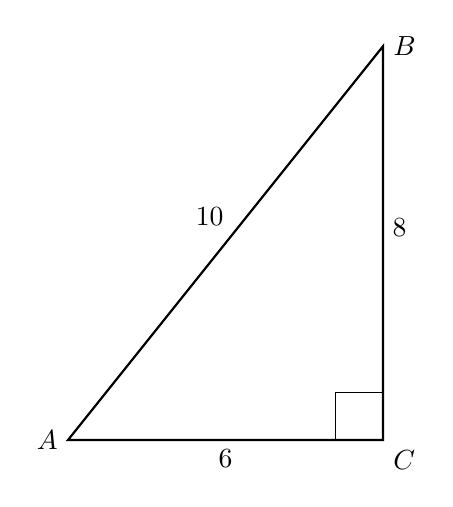
\begin{tikzpicture}[scale=1]
        \draw [thick]
        (0,0)node[left]{$A$}--
        (4,0)node[below right]{$C$}--
        (4,5)node[right]{$B$}--cycle;
        \draw (4,0)++(-0.6,0)--++(0,0.6)--+(0.6,0);
        \node at (2,0)[below]{$6$};
        \node at (4,2.7)[right]{$8$};
        \node at (1.8,2.6)[above]{$10$};
      \end{tikzpicture}
\end{flushright}
\end{multicols}

\item Use the tangent function to find the value of $BC=x$ for $\triangle ABC$ as shown.
  \begin{flushright}
    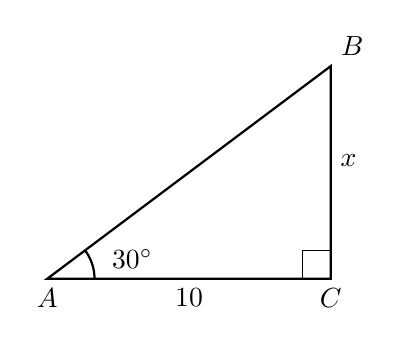
\begin{tikzpicture}[scale=0.6]
      \draw [thick](0,0)node[below]{$A$}--
      (6,0)node[below]{$C$}--
      (6,4.5)node[above right]{$B$}--cycle;
      \draw (6,0)++(-0.6,0)--++(0,0.6)--+(0.6,0);
      \node at (3,0)[below]{$10$};
      \node at (6,2.5)[right]{$x$};
      \draw [thick, -] (1,0) arc [start angle=0, end angle=37, radius=1];
      \node at (1.8,0)[above]{$30^\circ$};
    \end{tikzpicture}
  \end{flushright} \vspace{2cm}

\item $\triangle ABC$ is shown with $m\angle C=90^\circ$. The lengths of the triangle's sides are $a$, $b$, and $c$. Express each trigonometric ratio as a fraction of two variables. \vspace{1cm}
\begin{multicols}{2}
    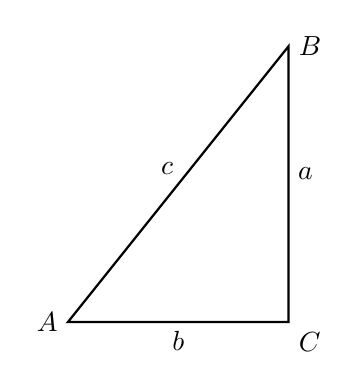
\begin{tikzpicture}[scale=0.7]
      \draw [thick]
      (0,0)node[left]{$A$}--
      (4,0)node[below right]{$C$}--
      (4,5)node[right]{$B$}--cycle;
      \node at (2,0)[below]{$b$};
      \node at (4,2.7)[right]{$a$};
      \node at (1.8,2.5)[above]{$c$};
    \end{tikzpicture}
      \begin{enumerate}
      \item $\sin B =$ \vspace{0.75cm}
      \item $\cos B =$ \vspace{0.75cm}
      \item $\tan B =$ \vspace{0.75cm}
    \end{enumerate}
\end{multicols}

\newpage
\item Given right $\triangle JKL$ with $\overline{JK} \perp \overline{KL}$, $JL=12.4$, $m\angle J=41^\circ$. Find the length $JK$, \emph{rounded to the nearest hundredth}.
  \begin{flushright}
    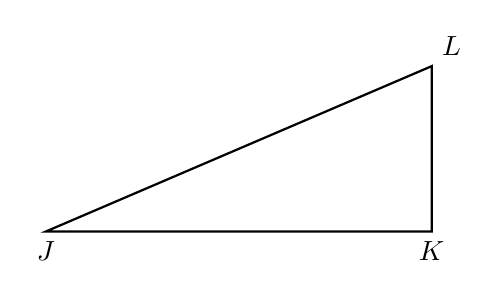
\begin{tikzpicture}[scale=0.7]
      \draw [thick]
      (0,0) node[below]{$J$}--
      (7,0)  node[below]{$K$}--
      (7,3) node[above right]{$L$}--cycle;
    \end{tikzpicture}
  \end{flushright} \vspace{1.5cm}

\item Right triangle $ABC$ is shown with $AB=20$, $m\angle A=33^\circ$. Find the value of $BC=x$.
  \begin{flushright}
    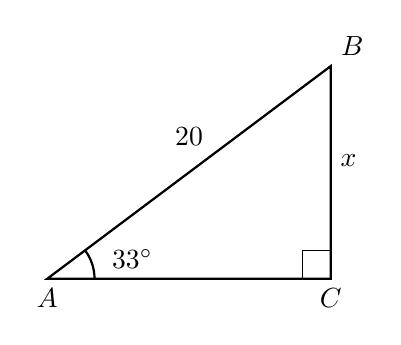
\begin{tikzpicture}[scale=0.6]
      \draw [thick](0,0)node[below]{$A$}--
      (6,0)node[below]{$C$}--
      (6,4.5)node[above right]{$B$}--cycle;
      \draw (6,0)++(-0.6,0)--++(0,0.6)--+(0.6,0);
      \node at (3,3){$20$};
      \node at (6,2.5)[right]{$x$};
      \draw [thick, -] (1,0) arc [start angle=0, end angle=37, radius=1];
      \node at (1.8,0)[above]{$33^\circ$};
    \end{tikzpicture}
  \end{flushright} \vspace{1.5cm}

\item Express the result to \emph{the nearest thousandth}.  \vspace{0.5cm}
\begin{multicols}{2}
  \begin{enumerate}
    \item $\sin 32^\circ = $ \vspace{1cm}
    \item $\cos 29^\circ =$
    \item $\cos 58^\circ = $ \vspace{1cm}
    \item $\sin 61^\circ =$
  \end{enumerate}
\end{multicols} \vspace{0.5cm}

\item Express the result to \emph{the nearest whole degree}.  \vspace{0.5cm}
\begin{multicols}{2}
  \begin{enumerate}
    \item $\sin^{-1} 0.420 = $ \vspace{1cm}
    \item $\cos^{-1} 0.675 =$
    \item $\cos^{-1} 0.850 = $ \vspace{1cm}
    \item $\sin^{-1} 0.125 =$
  \end{enumerate}
\end{multicols}

\end{enumerate}
\end{document}
  